\subsubsection{Linear and quadratic drifts}
\noindent
\par In our quality control analysis, we were interesting to remove the noise
from the BOLD images. The previous section explained how we select the voxels
that are in the brain. This section is dealing with noise motion. 

\noindent
\par Applying the mask on the image data allow us to select only the voxels that
are in the brain. 
We then model our signal with some additional drift terms to account for
the subject head motion in the scanner. We decide to add a linear and a 
quadratic drift terms as regressors. The following brain images justify
our design decision.

\begin{figure}[H]
\begin{subfigure}{.5\textwidth}
  \centering
  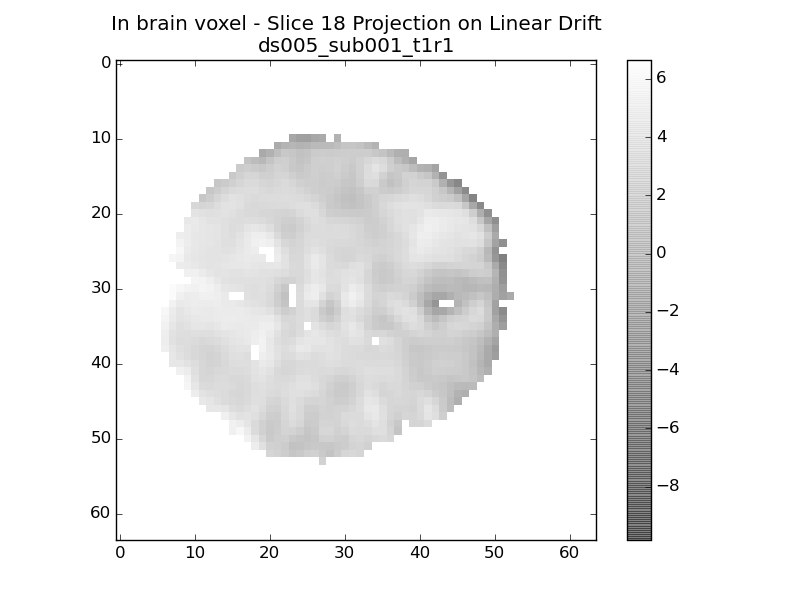
\includegraphics[width=.9\linewidth]{../fig/drifts/ds005_sub001_t1r1_withdrift_middleslice_5.png}
  \caption{Linear drift}
  \label{fig:drift1}
\end{subfigure}%
\begin{subfigure}{.5\textwidth}
  \centering
  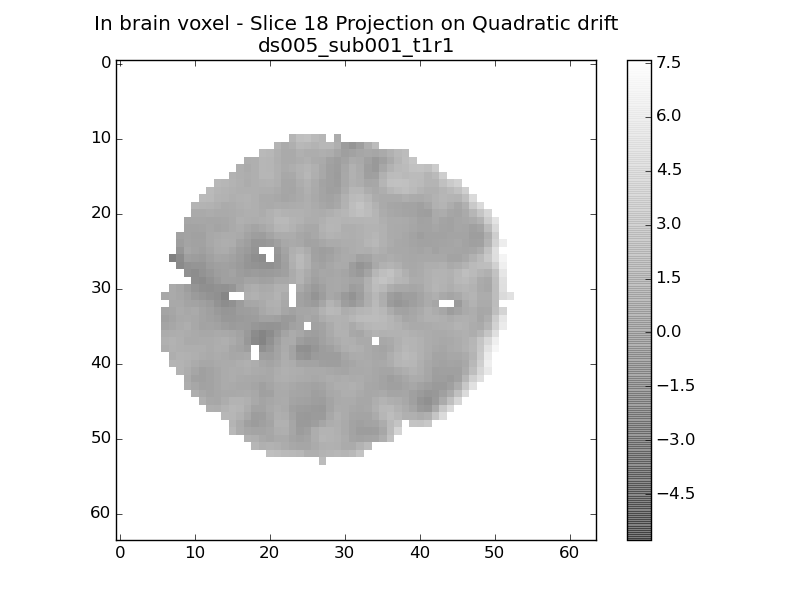
\includegraphics[width=.9\linewidth]{../fig/drifts/ds005_sub001_t1r1_withdrift_middleslice_6.png}
  \caption{Quadratic drift}
  \label{fig:drift2}
\end{subfigure}
\caption{Projection of the brain image on the drift regressors - subject1 - run1}
\label{fig:drifta}
\end{figure}

The above image illustrates the effect of the linear drift regressor on the BOLD image.
Lighter pixels indicate a higher position of the zone compare
to darker zones. We can clearly see the edges of the top right of the brain to be
dark (black) and the edges on the bottom left of the brain to be light (white). 
This suggests a clear linear movement of the head in the direction of the axis. 

The above image clearly illustrates a strong influence on the quadratic regressor in
the design matrix. We can clearly distinguish light and dark areas on the above images.
Our design matrix includes the above drift regressors in order to get a more accurate
estimation of the actvaction of the task which effects will not be confounded with the 
motion of the brain.
The drift terms model gradual drifts across the time-series, but other parameters can
explain the variance in the data. The next section is aiming to find the principal 
components of the data that have the most variance.
